\iffalse
\let\negmedspace\undefined
\let\negthickspace\undefined
\documentclass[journal,12pt,twocolumn]{IEEEtran}
\usepackage{cite}
\usepackage{amsmath,amssymb,amsfonts,amsthm}
\usepackage{algorithmic}
\usepackage{graphicx}
\usepackage{textcomp}
\usepackage{xcolor}
\usepackage{txfonts}
\usepackage{listings}
\usepackage{enumitem}
\usepackage{mathtools}
\usepackage{gensymb}
\usepackage{comment}
\usepackage[breaklinks=true]{hyperref}
\usepackage{tkz-euclide} 
\usepackage{listings}
\usepackage{gvv}                                        
\def\inputGnumericTable{}                                 
\usepackage[latin1]{inputenc}                                
\usepackage{color}                                            
\usepackage{array}                                            
\usepackage{longtable}                                       
\usepackage{calc}                                             
\usepackage{multirow}                                         
\usepackage{hhline}                                           
\usepackage{ifthen}                                           
\usepackage{lscape}

\newtheorem{theorem}{Theorem}[section]
\newtheorem{problem}{Problem}
\newtheorem{proposition}{Proposition}[section]
\newtheorem{lemma}{Lemma}[section]
\newtheorem{corollary}[theorem]{Corollary}
\newtheorem{example}{Example}[section]
\newtheorem{definition}[problem]{Definition}
\newcommand{\BEQA}{\begin{eqnarray}}
\newcommand{\EEQA}{\end{eqnarray}}
\newcommand{\define}{\stackrel{\triangle}{=}}
\theoremstyle{remark}
\newtheorem{rem}{Remark}

\begin{document}

\bibliographystyle{IEEEtran}
\vspace{3cm}
\title{\textbf{10.05.2.3}}
\author{EE23BTECH11053-R.Rahul$^{*}$% <-this % stops a space
}

\maketitle
\textbf{QUESTION:}
\\
1. In the following APs, find the missing terms in the boxes:\\
(i) 2,\textunderscore, 26 \\
(ii) \textunderscore, 13,\textunderscore , 3\\
(iii)  5,  \textunderscore, \textunderscore,9\(\frac{1}{2}\) \\
(iv) - 4, \textunderscore,  \textunderscore, \textunderscore, \textunderscore, 6\\
(v)  \textunderscore,38, \textunderscore, \textunderscore, \textunderscore, '- 22'\\

\solution
\fi
\begin{table}[h]
  \centering
  \renewcommand{\arraystretch}{1.5}
\begin{tabular}{|c|c|c|}
\hline
Parameter & Description \\\hline
\( n \) & No. of terms in the A.P  \\\hline
\(x(0) \) & first term in the A.P \\\hline
\( d \) & common difference in the A.P  \\\hline
\(x(n)=x(0)+nd\) & $(n+1)^{th}$ term in A.P\\ \hline
\end{tabular}
\caption{variables}
\end{table}


\begin{center}
\begin{enumerate}
    \item  
     \begin{align}
          26&=2+2d\\
        24&=2d \\
        \therefore d&=12\\
         x(1)&=14
     \end{align}
     The $Z$-transform of $x(n) = (2 + 12n)u(n)$ is given by:
     \begin{align}
    X(z)&=\frac{2+{10z^{-1}}}{(1-{z^{-1}})^2} \qquad|z|>1  \notag\\
     \end{align}     
     \item       
      \begin{align}
         3-13&=2d\\
           -10&=2d\\
           \therefore d&=-5\\
            x(1)&=18\\
            x(2)&=8
      \end{align}
     The $Z$-transform of $x(n) = (18 - 5n)u(n)$ is given by:
\begin{align}
    &X(z)=\frac{18-{23z^{-1}}}{(1-{z^{-1}})^2} \qquad  |z|>1  \notag\\
\end{align}
       \item    
     \begin{align}
           9\ \frac{1}{2}\ &=5+3d \\
           3d&=\frac{9}{2}\\
           \therefore d&=\frac{3}{2}\ \\ 
          x(1)&=6\ \frac{1}{2}\\
          x(2)&=8
     \end{align}
     $Z$-transform of $x(n) = (5 + \frac{3}{2}n)u(n)$ is given by:
\begin{align}
    &X(z)=\frac{5-\frac{7}{2}{z^{-1}}}{(1-{z^{-1}})^2} \qquad |z|>1 \notag\\
\end{align}
      \item       
    \begin{align}
     6&=-4+5d\\
     10&=5d\\
     \therefore d&=2\\
          x(1)&=-2\\
          x(2)&=0\\
          x(3)&=2 \\
          x(4)&=4 \notag\\
    \end{align}
    $Z-transform of x(n) = (-4 + 2n)u(n) $is given by:
    \begin{align}
       &X(z)=\frac{-4+6{z^{-1}}}{(1-{z^{-1}})^2} \qquad  |z|>1  \notag\\
    \end{align}
       \item    
     \begin{align}
         -22-38&=4d\\
          -60&=4d\\
           \therefore d&=-15\\
            x(0)&=53\\
            x(2)&=23\\
            x(3)&=8\\
            x(4)&=-7 \notag\\
     \end{align}
     $Z$-transform of $x(n) = (53 - 15n)u(n)$ is given by:
\begin{align}
       &X(z)=\frac{53-68{z^{-1}}}{(1-{z^{-1}})^2}\qquad|z|>1 \notag \\
\end{align}
\end{enumerate}             
          
\end{center}

\begin{figure}[h]
       \centering
        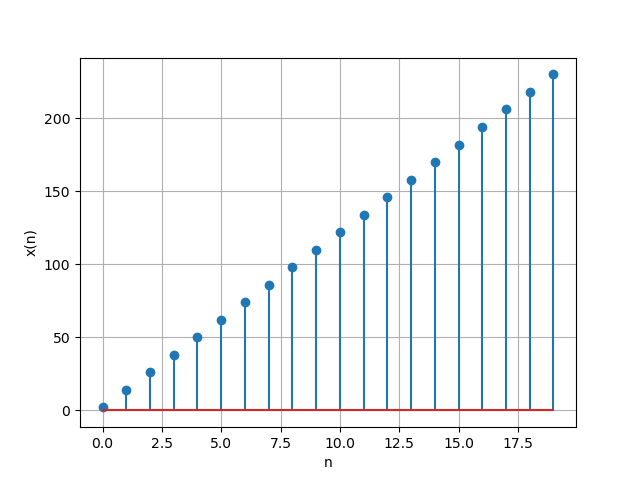
\includegraphics[width=1\linewidth]{ncert-maths/10/5/2/3/figs/plot1.png} % Adjust the width as needed
        \caption{}
\end{figure}

\begin{figure}[h]
      \centering
       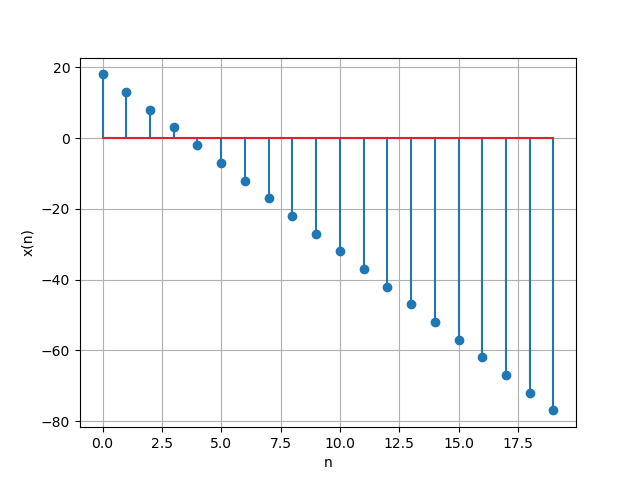
\includegraphics[width=1\linewidth]{ncert-maths/10/5/2/3/figs/plot2.png} % Adjust the width as needed
        \caption{}
    \end{figure}
    
\begin{figure}[h]
      \centering
       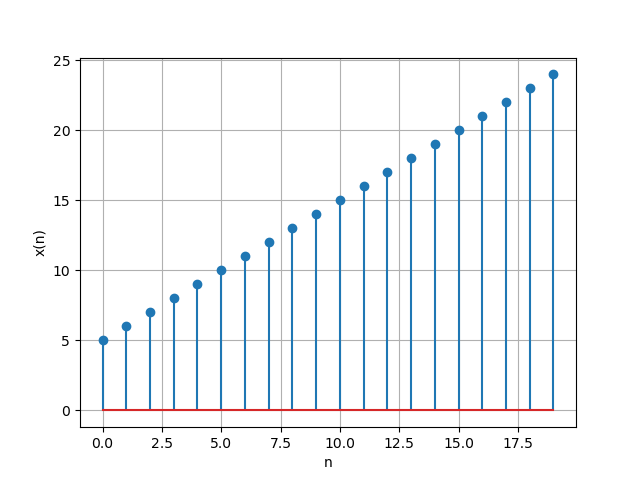
\includegraphics[width=1\linewidth]{ncert-maths/10/5/2/3/figs/plot3.png} % Adjust the width as needed
        \caption{}
    \end{figure}
    
\begin{figure}[h] 
      \centering
       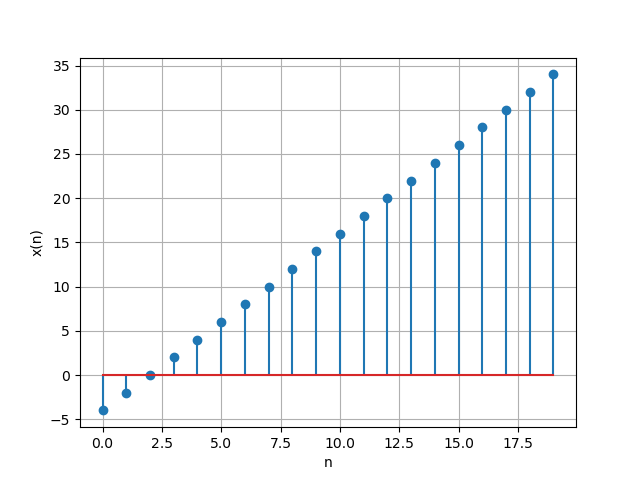
\includegraphics[width=1\linewidth]{ncert-maths/10/5/2/3/figs/plot4.png} % Adjust the width as needed
        \caption{}
    \end{figure}
    
\begin{figure}[h]
      \centering
       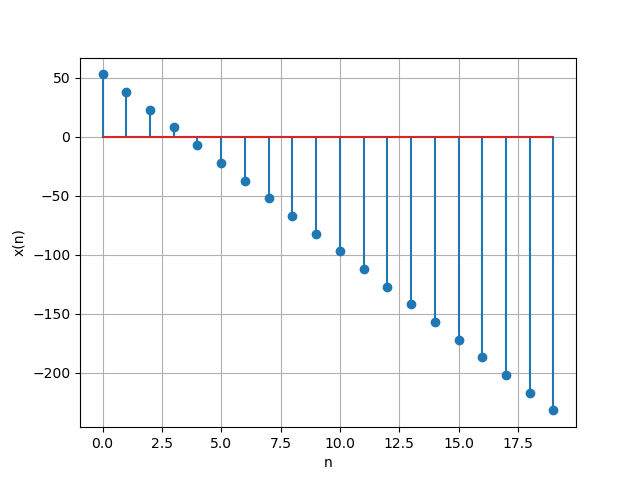
\includegraphics[width=1\linewidth]{ncert-maths/10/5/2/3/figs/plot5.png} % Adjust the width as needed
        \caption{}
\end{figure}
%\end{document}
